\section{tasks::flatfield Class Reference}
\label{classtasks_1_1flatfield}\index{tasks::flatfield@{tasks::flatfield}}
Inheritance diagram for tasks::flatfield::\begin{figure}[H]
\begin{center}
\leavevmode
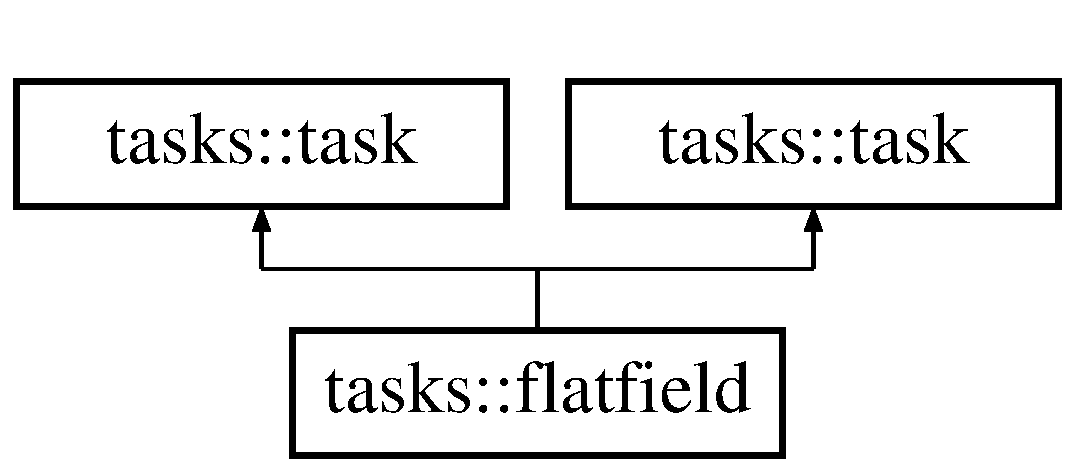
\includegraphics[height=2cm]{classtasks_1_1flatfield}
\end{center}
\end{figure}
\subsection*{Public Member Functions}
\begin{CompactItemize}
\item 
def \textbf{run}\label{classtasks_1_1flatfield_1192e37528e19d117edb8c848d1f0dfe}

\item 
def \textbf{run}\label{classtasks_1_1flatfield_1192e37528e19d117edb8c848d1f0dfe}

\end{CompactItemize}
\subsection*{Static Public Attributes}
\begin{CompactItemize}
\item 
string \textbf{name} = '{\bfflatfield}'\label{classtasks_1_1flatfield_70eecd05a653f468f017ec9c5adc7088}

\item 
string \textbf{button\-Text} = 'Divide by 2-D flat'\label{classtasks_1_1flatfield_7d5399128a9f975eb6f00212ee217ca9}

\item 
string \textbf{suffix} = 'flat'\label{classtasks_1_1flatfield_585d924d4d2d46488922ce09b3446ebe}

\item 
list \textbf{prereq} = ['{\bfpreproc}']\label{classtasks_1_1flatfield_ad4259bdcad744f1cc6cc1ae9a4d3e2e}

\end{CompactItemize}


\subsection{Detailed Description}


\footnotesize\begin{verbatim}Divide by 2-dimensional normalized FLAT.
\end{verbatim}
\normalsize
 



The documentation for this class was generated from the following files:\begin{CompactItemize}
\item 
old/PANICtool-1.0/tasks.py\item 
old/tasks.py\end{CompactItemize}
